\documentclass[12pt,a4paper,twoside]{report}
% -------------------------------------------------------------------- %
% Pacotes

\usepackage[utf8]{inputenc}
\usepackage[T1]{fontenc}
\usepackage[brazil]{babel}
\usepackage[fixlanguage]{babelbib}
\usepackage[pdftex]{graphicx}      % usamos arquivos pdf/png como figuras
\usepackage{setspace}              % espaçamento flexvel
\usepackage{indentfirst}           % indentação do primeiro parágrafo
\usepackage{makeidx}               % índice remissivo
\usepackage[nottoc]{tocbibind}     % acrescentamos a bibliografia/indice/conteudo no Table of Contents
\usepackage{courier}               % usa o Adobe Courier no lugar de Computer Modern Typewriter
\usepackage{type1cm}               % fontes realmente escaláveis
\usepackage{titletoc}
\usepackage{ucs}
\usepackage[font=small,format=plain,labelfont=bf,up,textfont=it,up]{caption}
\usepackage[usenames,svgnames,dvipsnames]{xcolor}
\usepackage[a4paper,top=2.54cm,bottom=2.0cm,left=2.0cm,right=2.54cm]{geometry} % margens
\usepackage{amsmath}

\usepackage[pdftex,plainpages=false,pdfpagelabels,pagebackref,colorlinks=true,citecolor=DarkGreen,
linkcolor=NavyBlue,urlcolor=DarkRed,filecolor=green,bookmarksopen=true]{hyperref} % links coloridos
\usepackage[all]{hypcap}                % soluciona o problema com o hyperref e capítulos
\usepackage[square,sort,nonamebreak,comma]{natbib}  % citação bibliográfica alpha
\fontsize{60}{62}\usefont{OT1}{cmr}{m}{n}{\selectfont}
\usepackage{upquote}                    % formata apóstrofes '
\usepackage{textcomp}

% Para formatar corretamente as URLs
\usepackage{url}
% -------------------------------------------------------------------- %
% Cabeçalhos similares ao TAOCP de Donald E. Knuth
\usepackage{fancyhdr}
\pagestyle{fancy}
\fancyhf{}
\renewcommand{\chaptermark}[1]{\markboth{\MakeUppercase{#1}}{}}
\renewcommand{\sectionmark}[1]{\markright{\MakeUppercase{#1}}{}}
\renewcommand{\headrulewidth}{0pt}

% -------------------------------------------------------------------- %
\graphicspath{{./img/}}        % caminho das figuras
\frenchspacing                     % arruma o espaço: id est (i.e.) e exempli gratia (e.g.)
\urlstyle{same}                    % URL com o mesmo estilo do texto e no mono-spaced
\makeindex                         % para o índice remissivo
\raggedbottom                      % para no permitir espaços extras no texto
\fontsize{60}{62}\usefont{OT1}{cmr}{m}{n}{\selectfont}
\cleardoublepage
\normalsize

% -------------------------------------------------------------------- %
% Cores para formatação de código
\usepackage{color}
\definecolor{vermelho}{rgb}{0.6,0,0} % para strings
\definecolor{verde}{rgb}{0.25,0.5,0.35} % para comentários
\definecolor{roxo}{rgb}{0.5,0,0.35} % para palavras-chaves
\definecolor{azul}{rgb}{0.25,0.35,0.75} % para strings
\definecolor{cinza-claro}{gray}{0.95}
% -------------------------------------------------------------------- %
% Opções de listagem usados para o código fonte
% Ref: http://en.wikibooks.org/wiki/LaTeX/Packages/Listings



\usepackage{listings}           % para formatar código-fonte (ex. em Java)


\lstset{ %
language=[Objective]Caml,  % seleciona a linguagem do código (aqui em lstlang0.sty
basicstyle=\footnotesize\ttfamily, % o tamanho da fonte usado no código
commentstyle=\color{verde}\bfseries,  % formatação de comentários
stringstyle=\color{azul},    % formatação de strings
upquote=true,
numbers=left,                   % onde colocar os números de linha
numberstyle=\tiny,  % o tamanho da fonte usada para a numeração das linhas
stepnumber=1,                   % o intervalo entre dois números de linhas. Se for 1, numera cada uma.
numbersep=5pt,                  % how far the line-numbers are from the code
showspaces=false,               % show spaces adding particular underscores
showstringspaces=false,         % underline spaces within strings
showtabs=false,                 % show tabs within strings adding particular underscores
keywordstyle=\color{roxo}\bfseries,
keywordstyle=[1]\color{roxo}\bfseries,
keywordstyle=[2]\color{verde}\bfseries,
%        keywordstyle=[3]\textbf,    %
%        keywordstyle=[4]\textbf,   \sqrt{\sqrt{}} %
frame=b,                   % adds a frame around the code
framerule=0.6pt,
tabsize=2,                      % sets default tabsize to 2 spaces
captionpos=t,                   % sets the caption-position to top
breaklines=true,                % sets automatic line breaking
breakatwhitespace=false,        % sets if automatic breaks should only happen at whitespace
escapeinside={\%*}{*)},         % if you want to add a comment within your code
backgroundcolor=\color[rgb]{1.0,1.0,1.0}, % choose the background color.
rulecolor=\color[rgb]{0.8,0.8,0.8},
extendedchars=true,
xleftmargin=10pt,
xrightmargin=10pt,
framexleftmargin=10pt,
framexrightmargin=10pt,
literate={â}{{\^{a}}}1  % para formatar corretamente os acentos do Português ao usar utf8
    {ê}{{\^{e}}}1
    {ô}{{\^{o}}}1
    {Â}{{\^{A}}}1
    {Ê}{{\^{E}}}1
    {Ô}{{\^{O}}}1
    {á}{{\'{a}}}1
    {é}{{\'{e}}}1
    {í}{{\'{i}}}1
    {ó}{{\'{o}}}1
    {ú}{{\'{u}}}1
    {Á}{{\'{A}}}1
    {É}{{\'{E}}}1
    {Í}{{\'{I}}}1
    {Ó}{{\'{O}}}1
    {Ú}{{\'{U}}}1
    {à}{{\`{a}}}1
    {À}{{\`{A}}}1
    {ã}{{\~{a}}}1
    {õ}{{\~{o}}}1
    {Ã}{{\~{A}}}1
    {Õ}{{\~{O}}}1
    {ç}{{\c{c}}}1
    {Ç}{{\c{C}}}1
    {ü}{{\"u}}1
    {Ü}{{\"U}}1
}

\renewcommand{\lstlistingname}{Listagem}
\renewcommand{\lstlistlistingname}{Lista de Listagens}

% Definição de novos estilos
\lstdefinestyle{Bash}
    {language=bash,frame=single,numbers=none,basicstyle=\footnotesize\ttfamily,
     morekeywords={cp,mkdir,sudo,tar}}

% Definição de novos ambientes
\lstnewenvironment{terminal}
  {\lstset{style=Bash}}
  {}

\lstnewenvironment{ocaml}
  {\lstset{basicstyle=\scriptsize\ttfamily,
           frame=single,
           frameround=tttt,
           framerule=2pt,
           numbers=none,
           rulecolor=\color{Salmon}}}
  {}

\lstnewenvironment{xml}
   {\lstset{language=XML,frame=single,numbers=none}}
   {}

\lstnewenvironment{interprete}
  {\lstset{frame=single,
            frameround=tttt,
            numbers=none,
            basicstyle=\ttfamily,
            framerule=2pt,
            rulecolor=\color{CadetBlue}}}
  {}
% Formata o caption da listagem
% \DeclareCaptionFont{blue}{\color{blue}}

% \captionsetup[lstlisting]{singlelinecheck=false, labelfont={blue}, textfont={blue}}
\usepackage{caption}
\DeclareCaptionFont{white}{\color{white}}
\DeclareCaptionFormat{listing}{\colorbox[cmyk]{0.43, 0.35, 0.35,0.01}{\parbox{\textwidth}{\hspace{15pt}#1#2#3}}}
\captionsetup[lstlisting]{format=listing,labelfont=white,textfont=white, singlelinecheck=false, margin=0pt, font={bf,footnotesize}}

\newcommand{\ListingsPath}{./codigos}
% Inclui o nome do arquivo como Caption
\newcommand{\filelisting}[2][]{%
    \lstinputlisting[caption={\texttt{\detokenize{#2}}},#1]{\ListingsPath/#2}%
}

% ---------------------------------------------------------------------------- %

% ---------------------------------------------------------------------------- %

\title{Construção de um Compilador de códigos Java para Parrot Virtual Machine}
\date{}
\author{Frederico Franco Calhau \\
\texttt{\small \url{fred_ffc@hotmail.com}}
\vspace{1cm} \\
Faculdade de Computação \\
Universidade Federal de Uberlândia
}
\date{\today}

%\includeonly{cap-clojure,magical,short}
\begin{document}
  \maketitle
% -------------------------------------------------------------------- %
% Listas de figuras, tabelas e códigos criadas automaticamente
\listoffigures
\listoftables
\lstlistoflistings
% -------------------------------------------------------------------- %

% -------------------------------------------------------------------- %
% Sumário
\tableofcontents

% Capítulos do trabalho

% cabeçalho para as páginas de todos os capítulos
\fancyhead[RE,LO]{\thesection}

%\singlespacing              % espaçamento simples
\setlength{\parskip}{0.15in} % espaçamento entre paragráfos

\chapter{Introdução}

Este relatório possui o propósito de documentar as atividades realizadas ao longo da disciplina de Construção de Compiladores, a qual tem como objetivo - que também pode ser facilmente deduzido pelo seu nome – de construir uma versão simples de um compilador.

Assim, esse trabalho consiste em criar tal compilador que seja capaz de compilar códigos escritos em Mini Java (um subconjunto da linguagem Java) e "transformá-los" na linguagem PASM (Parrot Assembly), a qual poderá ser interpretada pela máquina virtual Parrot. Para construir esse compilador, utilizou-se a linguagem de programação OCaml, e o sistema operacional macOS (10.12.2).

A seguir, encontra-se algumas explicações das tecnologias e termos descritos acima.

\section{Instalação dos componentes via Homebrew}

Homebrew é um gerenciador de pacotes para macOS, escrito em Ruby, e é responsável por instalar pacotes nos diretórios adequados e fazer adequadamente a configuração desses pacotes, instalá-lo facilita todo o processo de instalação dos componentes necessários.

Para instalar o homebrew basta digitar no terminal:

\begin{terminal}
$ /usr/bin/ruby -e "\$(curl -fsSL https://raw.githubusercontent.com/Homebrew/install/master/install)"
\end{terminal}

\subsection{Instalando Ocaml}

Novamente através do homebrew, basta digitar:

\begin{terminal}
$ brew install ocaml
\end{terminal}

Resultado:

\begin{figure}[!ht]
\centering
\caption{Instalando e testando OCaml}
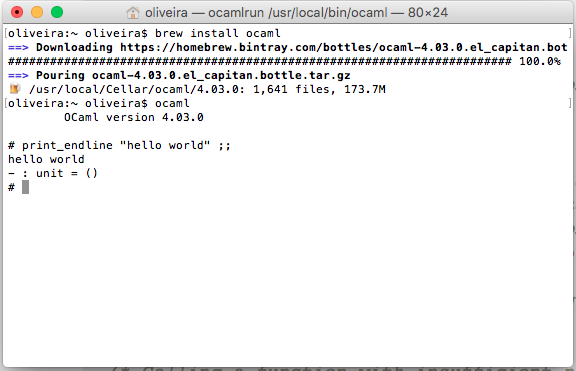
\includegraphics[scale=0.27]{img/brew-ocaml.png}
\end{figure}

\subsection{Instalação da Parrot VM}

Digitar no Terminal:
\begin{terminal}
$ brew install parrot
\end{terminal}

Resultado:
\begin{figure}[!ht]
\centering
\caption{Instalando e testando Parrot}
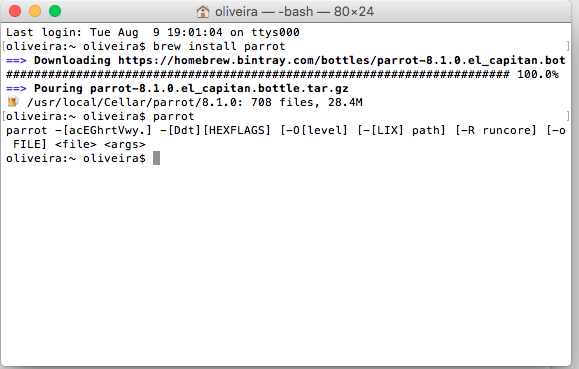
\includegraphics[scale=0.27]{img/brew-parrot.png}
\end{figure}

\section{Máquina Virtual Parrot}

Parrot é uma máquina virtual (VM) projetada para atender as necessidades de linguagens tipadas dinamicamente (como por exemplo Perl e Python), e para prover interoperabilidade entre essas linguagens aceitas.

Ela é uma máquina baseada em registradores, e há 4 tipos desses: inteiros (I), números (N), palavras (S), e PMCs (P). A quantidade de registradores necessários é determinada para cada sub-rotina em tempo de compilação. Os registradores serão nomeados da seguinte maneira "XN" onde 'X' seria uma das letras que representa o tipo do registrador, e 'N' um número entre 0 e a quantidade máxima de registradores daquele tipo. Assim, o quinto registrador do tipo inteiro se chamaria: "I4".

Os registradores do tipo PMCs (Polymorphic Container) representam qualquer tipo ou estrutura de dados complexa (classes e objetos), incluindo agregações de tipos (vetores, hash tables, etc). Eles podem implementar seu próprio comportamento para operações aritméticas, lógicas, e que envolvam palavras, oferecendo comportamento específico para cada linguagem. Podem também ser carregados dinamicamente quando forem requisitados, ao invés de serem montados estaticamente junto ao executável Parrot.

Atualmente, a VM Parrot aceita instruções descritas de 4 formas diferentes, as quais serão descritas a seguir em ordem de abstração –– da mais abstrata (high-level) para a mais próxima da linguagem da máquina (low-level):

\begin{itemize}
    \item PIR (Parrot Intermediate Representation) é a forma padrão. Como o próprio nome diz, ela é uma linguagem intermediária que esconde alguns detalhes low-level do usuário, mas que será convertida para PASM;
    \item PASM (Parrot Assembly) é um assembly customizado para a máquina Parrot. Utilizaremos essa linguagem;
    \item PAST (Parrot Abstract Syntax Tree) linguagem útil para construção de compiladores porque permite receber como entrada uma árvore sintática abstrata;
    \item PBC (Parrot Bytecode) é a linguagem de máquina que pode ser executada imediatamente. Todas as outras linguagens serão primeiro convertidas em PBC para assim poderem ser executadas eficientemente pela máquina Parrot.
\end{itemize}

Ao longo deste relatório, a linguagem PASM será utilizada como linguagem alvo da nossa compilação, uma vez que ela se assemelha mais com as linguagens (assembly) aceitas pelas outras plataformas estudadas por outros alunos. No entanto, infelizmente, os compiladores de Parrot disponíveis atualmente conseguem apenas compilar para a linguagem PIR.


Fazendo alguns testes com PASM e PIR:
\lstinputlisting[caption={Output Simples em Parrot Assembly Language}]{codigos/parrot/news.txt}
Para executar o código:
\begin{terminal}
$ parrot news.txt
\end{terminal}

\lstinputlisting[caption={Output Simples em Parrot Intermediate Representation}]{codigos/parrot/hello.txt}
Para executar o código:
\begin{terminal}
$ parrot hello.txt
\end{terminal}

Os arquivos PASM e PIR são convertidos para Parrot Bytecode (PBC) e somente então são executados pela máquina virutal, é possível obter o arquivo .pbc através comando:
\begin{terminal}
$ parrot -o output.pbc input.txt
\end{terminal}

De acordo com a documentação oficial, o Compilador Intermediário de Parrot é capaz de traduzir códigos PIR para PASM através do comando:

\begin{terminal}
$ parrot -o output.txt input.txt
\end{terminal}

Mas, infelizmente, essa execução resultou em um código bytecode (PBC), ao invés do assembly (PASM). Por isso, para analisar os códigos em PASM, será necessário "compilar" manualmente os arquivos fontes.

Apesar da documentação oficial enfatizar que a linguagem intermediária PIR ser mais recomendada e utilizada no desenvolvimento de ferramentas para Parrot, o alvo será a linguagem Assembly PASM.


\section{Parrot Assembly Language (PASM)}

A linguagem PASM é muito similar a um assembly tradicional, com exceção do fato de que algumas instruções permitem o acesso a algumas funções dinâmicas de alto nível do sistema Parrot.

Para melhor entender o funcionamento da linguagem PASM, compilaremos programas simples em Mini Java para PASM. No entanto, infelizmente, essa compilação será feita manualmente devido ao problema comentado anteriormente em que os compiladores disponíveis para a plataforma Parrot não geram mais códigos escritos em PASM, apenas em PIR.


\subsection{Códigos Java e PASM}

\subsubsection{Nano Programas}
\subsubsection{Nano 01}
\lstinputlisting[caption={Programa nano 01 em Java}]{codigos/nano01/nano01.java}
\lstinputlisting[caption={Programa nano 01 em PASM}]{codigos/nano01/nano01.txt}

\subsubsection{Nano 02}
\lstinputlisting[caption={Programa nano 02 em Java}]{codigos/nano02/nano02.java}
\lstinputlisting[caption={Programa nano 02 em PASM}]{codigos/nano02/nano02.txt}

\subsubsection{Nano 03}
\lstinputlisting[caption={Programa nano 03 em Java}]{codigos/nano03/nano03.java}
\lstinputlisting[caption={Programa nano 03 em PASM}]{codigos/nano03/nano03.txt}

\subsubsection{Nano 04}
\lstinputlisting[caption={Programa nano 04 em Java}]{codigos/nano04/nano04.java}
\lstinputlisting[caption={Programa nano 04 em PASM}]{codigos/nano04/nano04.txt}

\subsubsection{Nano 05}
\lstinputlisting[caption={Programa nano 05 em Java}]{codigos/nano05/nano05.java}
\lstinputlisting[caption={Programa nano 05 em PASM}]{codigos/nano05/nano05.txt}
Saída:
\begin{terminal}
2
\end{terminal}

\subsubsection{Nano 06}
\lstinputlisting[caption={Programa nano 06 em Java}]{codigos/nano06/nano06.java}
\lstinputlisting[caption={Programa nano 06 em PASM}]{codigos/nano06/nano06.txt}
Saída:
\begin{terminal}
-1
\end{terminal}

\subsubsection{Nano 07}
\lstinputlisting[caption={Programa nano 07 em Java}]{codigos/nano07/nano07.java}
\lstinputlisting[caption={Programa nano 07 em PASM}]{codigos/nano07/nano07.txt}
Saída:
\begin{terminal}
1
\end{terminal}

\subsubsection{Nano 08}
\lstinputlisting[caption={Programa nano 08 em Java}]{codigos/nano08/nano08.java}
\lstinputlisting[caption={Programa nano 08 em PASM}]{codigos/nano08/nano08.txt}
Saída:
\begin{terminal}
1
\end{terminal}

\subsubsection{Nano 09}
%\lstinputlisting[caption={Programa nano 09 em Java}]{codigos/nano09/nano09.java}
\lstinputlisting[caption={Programa nano 09 em PASM}]{codigos/nano09/nano09.txt}
Saída:
\begin{terminal}
1
\end{terminal}

\subsubsection{Nano 10}
\lstinputlisting[caption={Programa nano 10 em Java}]{codigos/nano10/nano10.java}
\lstinputlisting[caption={Programa nano 10 em PASM}]{codigos/nano10/nano10.txt}
Saída:
\begin{terminal}
0
\end{terminal}

\subsubsection{Nano 11}
\lstinputlisting[caption={Programa nano 11 em Java}]{codigos/nano11/nano11.java}
\lstinputlisting[caption={Programa nano 11 em PASM}]{codigos/nano11/nano11.txt}
Saída:
\begin{terminal}
3
5
\end{terminal}

\subsubsection{Nano 12}
\lstinputlisting[caption={Programa nano 12 em Java}]{codigos/nano12/nano12.java}
\lstinputlisting[caption={Programa nano 12 em PASM}]{codigos/nano12/nano12.txt}
Saída:
\begin{terminal}
0
0
0
0
\end{terminal}

\subsection{Micro Programas}
\subsubsection{Micro 01}
\lstinputlisting[caption={Programa micro 01 em Java}]{codigos/micro01/micro01.java}
\lstinputlisting[caption={Programa Micro 01 em PASM}]{codigos/micro01/micro01.txt}
\begin{terminal}
Celsius -> Fahrenheit
Digite a Temperatura em Celsius: 20
A nova temperatura e: 68 graus F.
\end{terminal}

\subsubsection{Micro 02}
\lstinputlisting[caption={Programa micro 02 em Java}]{codigos/micro02/micro02.java}
\lstinputlisting[caption={Programa Micro 02 em PASM}]{codigos/micro02/micro02.txt}
\begin{terminal}
Digite o primeiro numero: 10
Digite o segundo numero: 20
o segundo numero e maior que o primeiro numero
Digite o primeiro numero: 20
Digite o segundo numero: 10
o primeiro numero e maior que o segundo numero
\end{terminal}

\subsubsection{Micro 03}
\lstinputlisting[caption={Programa micro 03 em Java}]{codigos/micro03/micro03.java}
\lstinputlisting[caption={Programa Micro 03 em PASM}]{codigos/micro03/micro03.txt}
\begin{terminal}
Digite um numero: 5
O numero nao esta no intervalo entre 100 e 200

Digite um numero: 150
O numero esta no intervalo entre 100 e 200

Digite um numero: 201
O numero nao esta no intervalo entre 100 e 200
\end{terminal}

\subsubsection{Micro 04}
\lstinputlisting[caption={Programa micro 04 em Java}]{codigos/micro04/micro04.java}
\lstinputlisting[caption={Programa Micro 04 em PASM}]{codigos/micro04/micro04.txt}
\begin{terminal}
Digite um numero: 50
Digite um numero: 50
Digite um numero: 50
Digite um numero: 50
Digite um numero: 50
Ao total foram digitados 5 numeros no intervalo entre 10 e 150.

Digite um numero: 02
Digite um numero: 03
Digite um numero: 25
Digite um numero: 60
Digite um numero: 160
Ao total foram digitados 2 numeros no intervalo entre 10 e 150.
\end{terminal}

\subsubsection{Micro 05}
\lstinputlisting[caption={Programa micro 05 em Java}]{codigos/micro05/micro05.java}
\lstinputlisting[caption={Programa Micro 05 em PASM}]{codigos/micro05/micro05.txt}
\begin{terminal}
H - Homem ou M - Mulher: H
H - Homem ou M - Mulher: M
H - Homem ou M - Mulher: H
H - Homem ou M - Mulher: M
H - Homem ou M - Mulher: M
Foram inseridos 2 homens
Foram inseridas 3 mulheres
\end{terminal}

\subsubsection{Micro 06}
\lstinputlisting[caption={Programa micro 06 em Java}]{codigos/micro06/micro06.java}
\lstinputlisting[caption={Programa Micro 06 em PASM}]{codigos/micro06/micro06.txt}
\begin{terminal}
Digite um numero de 1 a 5: 3
Tres
\end{terminal}

\subsubsection{Micro 07}
\lstinputlisting[caption={Programa micro 07 em Java}]{codigos/micro07/micro07.java}
\lstinputlisting[caption={Programa Micro 07 em PASM}]{codigos/micro07/micro07.txt}
\begin{terminal}
Digite um numero: 5
Positivo!
Deseja finalizar? (S/N): N
Digite um numero: -5
Negativo!
Deseja finalizar? (S/N): N
Digite um numero: 0
Zero!
Deseja finalizar? (S/N): S
\end{terminal}

\subsubsection{Micro 08}
\lstinputlisting[caption={Programa micro 08 em Java}]{codigos/micro08/micro08.java}
\lstinputlisting[caption={Programa Micro 08 em PASM}]{codigos/micro08/micro08.txt}
\begin{terminal}
Digite um numero: 50
O numero 50 e maior que 10.
Digite um numero: 5
O numero 5 e menor que 10.
Digite um numero: 0
O numero 0 e menor que 10.
\end{terminal}

\subsubsection{Micro 09}
\lstinputlisting[caption={Programa micro 09 em Java}]{codigos/micro09/micro09.java}
\lstinputlisting[caption={Programa Micro 09 em PASM}]{codigos/micro09/micro09.txt}
\begin{terminal}
Digite o preco: 10
Digite a venda: 10
O novo preco e: 11

Digite o preco: 40
Digite a venda: 600
O novo preco e: 46

Digite o preco: 90
Digite a venda: 1500
O novo preco e: 72
\end{terminal}

\subsubsection{Micro 10}
\lstinputlisting[caption={Programa micro 10 em Java}]{codigos/micro10/micro10.java}
\lstinputlisting[caption={Programa Micro 10 em PASM}]{codigos/micro10/micro10.txt}
\begin{terminal}
Digite um numero: 5
O fatorial de 5 e: 120
\end{terminal}

\subsubsection{Micro 11}
\lstinputlisting[caption={Programa micro 11 em Java}]{codigos/micro11/micro11.java}
\lstinputlisting[caption={Programa Micro 11 em PASM}]{codigos/micro11/micro11.txt}
\begin{terminal}
Digite um numero: 5
Positivo

Digite um numero: -5
Negativo

Digite um numero: 0
Zero
\end{terminal}


\clearpage
\addcontentsline{toc}{part}{Apêndice}
\appendix

\end{document}
